\subsection{Dance Dance Revolution}
Dance Dance Revolution (DDR) is a music video game series produced by Konami.
The series' gameplay involves the player using his or her feet to step on portions of a platform corresponding to arrows that appear on the screen to the beat of a song.
During gameplay arrows scroll across the screen (typically from the bottom of the screen and upwards), eventually passing over a set of stationary arrows before reaching the opposite end of the screen.
The game's objective is for the player to hit the corresponding arrows on the \textit{dance platform} when a scrolling arrow overlaps with the stationary arrows.
The player is given a judgment based on the accuracy which with they hit each note.
A sufficiently poor judgment will decrease the player's life bar.
The player's life bar reaching zero results in a game over.

\begin{figure}[h]
	\centering
	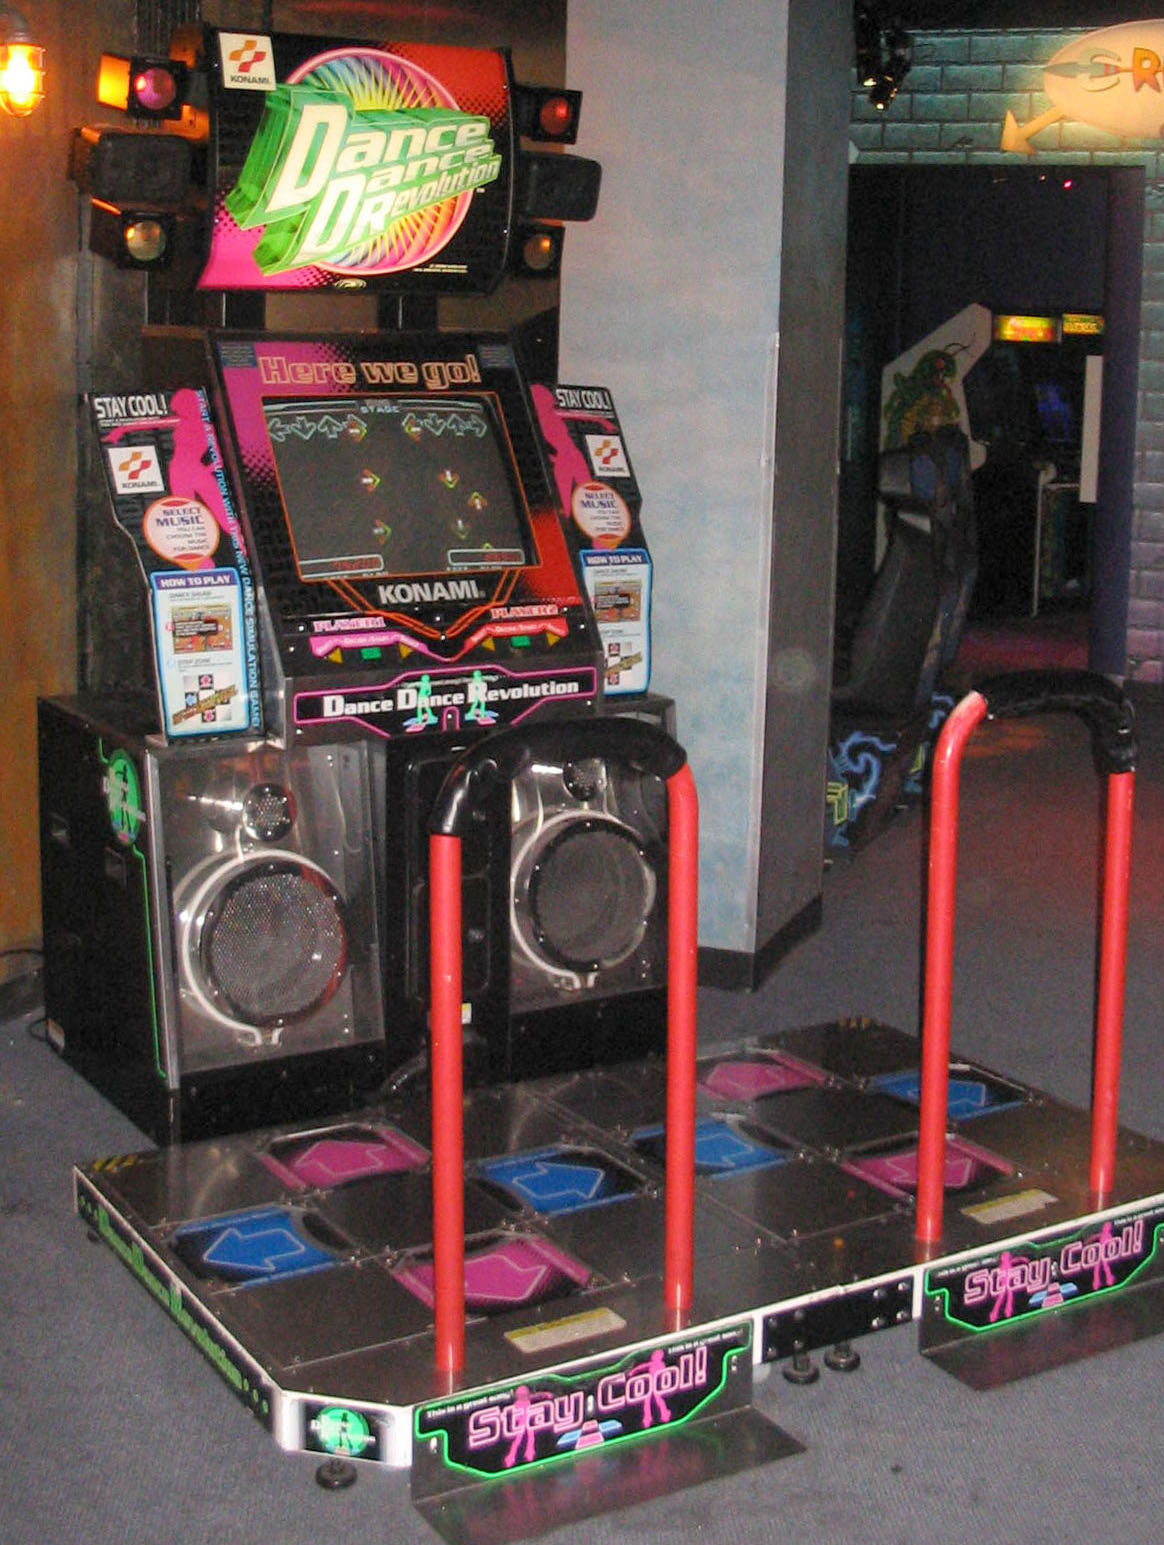
\includegraphics[width=2in]{{images/ddr3.jpg}}
	\caption{An original Dance Dance Revolution machine. Image courtesy of Poiuyt Man.}
	\label{img-ddr}
\end{figure}

\subsection{StepMania}
StepMania (SM) is a cross-platform open source rhythm video game which was developed as a Dance Dance Revolution simulator, released under the MIT license.
It allows for custom songs (known as ``Stepfiles'') and further modification of gameplay elements (such as the timing of judgments).
While originally developed as a DDR simulator, it is often played using a keyboard rather than a dance platform.

\begin{figure}[h]
	\centering
	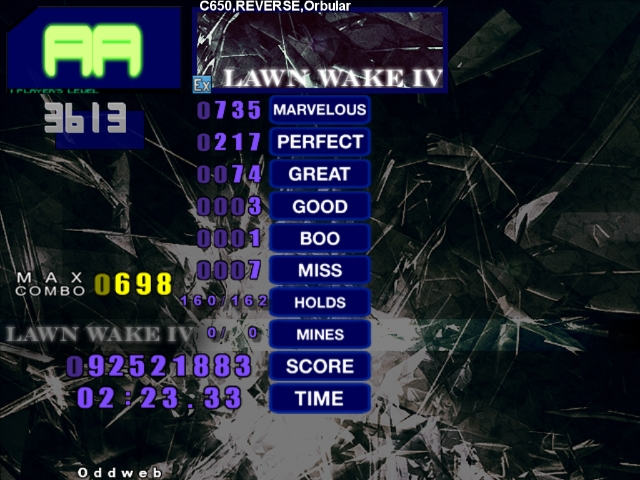
\includegraphics[width=4in]{{images/sm1.jpg}}
	\caption{A screenshot of a slightly modified StepMania 3.9 score screen. The song is Lawn Wake IV by The Flashbulb. Image courtesy of Oddweb.}
	\label{img-smss}
\end{figure}

Scoring in StepMania is based on judgments: each ``step'' (moving arrows) the player hits results in a judgment based on how far away the arrow is from the stationary arrows when the player ``hits'' it.
The closer the arrow is to the stationary arrows when it is hit, the better the judgment. 
A sufficiently poor judgment (or a complete miss) results in the player's life bar depleting.

\begin{figure}[h]
	\centering
	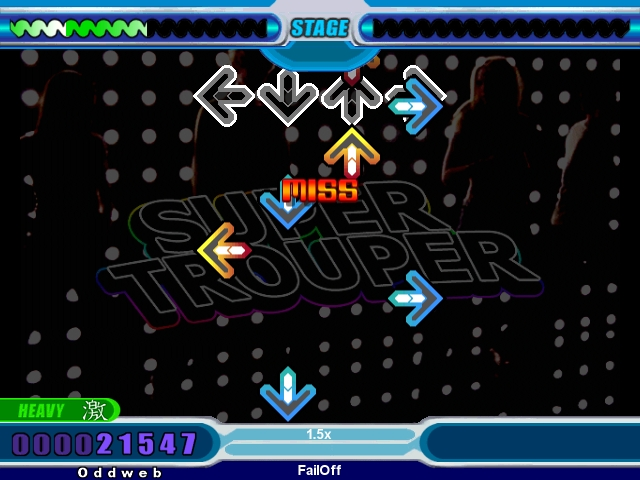
\includegraphics[width=4in]{{images/sm2.jpg}}
	\caption{A screenshot of a slightly modified StepMania 3.9 in-song interface, with the player having recently scored a ``perfect'' (the second best judgment in unmodified StepMania 3.9). The song is Super Trouper by A-Teens. Image courtesy of Oddweb.}
	\label{img-smgp}
\end{figure}

\subsection{Glossary}
The following is a list of terms used in relation to DDR/StepMania.
\begin{itemize}
	\item{\textbf{Arrows}: The arrows that scroll across to the rhythm of the song.}
	\item{\textbf{Stationary arrows}: The row of stationary shapes (or targets) the arrows approach.}
	\item{\textbf{Dance platform/mat}: A type of controller pressure sensitive areas that correspond to the arrows. See Figure~\ref{img-ddr}.}
	\item{\textbf{Song}: A ``song'' in StepMania includes the actual song/sound track and its steps.}
	\item{\textbf{Dance pattern}: Dance pattern: the set of arrows for a given song at a given difficulty.}
	\item{\textbf{Step}: All the arrows at a given time value (as in one step: one rearrangement of the feet on the dance platform). All arrows in a step have to be pressed within the step's time window for it to register as a hit.}
	\item{\textbf{Note}: Alternate name for ``step''.}
	\item{\textbf{Double}: A type of step containing two arrows.}
	\item{\textbf{Triples (trips)}: A step containing three arrows.}
	\item{\textbf{Quadruples (quads)}: A step containing four arrows.}
	\item{\textbf{Judgment}: A ``score'' given for each step hit.}
\end{itemize}